\section{Topología ferroviaria original}

	El primer ejemplo, ilustrado en la Figura \ref{fig:EJ8_1}, es una topología diseñada por el autor de la tesis, en base a dos líneas principales conectadas por un cambio de vías y seis cruces de vías. Los cambios de vías Sw11 y Sw12 permiten el intercambio de formaciones entre ambas vías principales. El objetivo de este ejemplo fue comprobar el funcionamiento del RNA con una topología de doble vía conectadas por dos cambios de vías, similares a las que se pueden encontrar en estaciones reales.
	
	\begin{figure}[h]
		\centering
		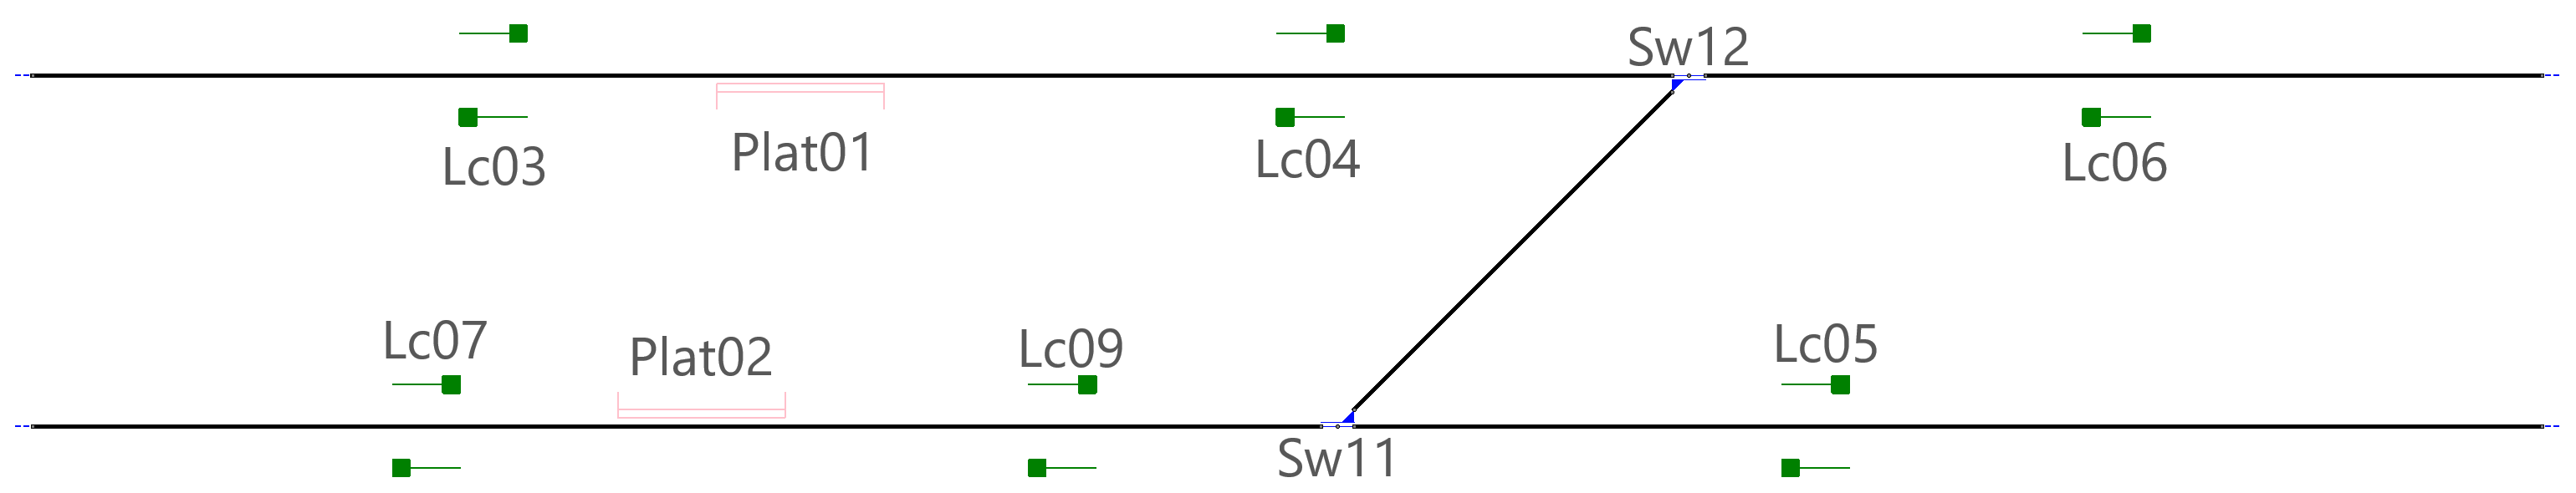
\includegraphics[width=1\textwidth]{resultados-obtenidos/ejemplo8/images/8_empty.png}
		\centering\caption{Topología ferroviaria del ejemplo 8 sin señalamiento.}
		\label{fig:EJ8_1}
	\end{figure}
	
	Para incrementar la dificultad del análisis y obtener resultados mas completos, todos los finales de vías son relativos y se añadieron las plataformas (Platform01, Platform02) y cruces de vías (Lc03, Lc04, Lc05, Lc06, Lc07, LC09). La infraestructura se distribuyó de forma tal de tener que en algunos casos el espacio entre ambos fuese suficiente (LevelCrossing04 y Platform01) y en otros no (LevelCrossing07 y Platform02).
